
\section{Results}
\label{section:results}
% In the simulation, the distance between dual-microphones is 14cm, and audio sampling rate is 48kHz. 
% All the statistics are run more than 3000 times for high confidence, and reported by Root Mean Square Error (RMSE).
% The parameter $\sigma$ in robust ThunderLoc has little impact to the localization performance. In default, $\sigma=1$.
\subsection{2D Simulation}
In this section, we evaluated our localization methods in 2D scenario using MATLAB.  
In the simulation, we randomly deployed dual-microphone mobile phones on a 10km $\times$ 10km area with uniform distribution, and the distance between dual-microphones is 14cm, and audio sampling rate is 48kHz. 
All the statistics are run more than 3000 times for high confidence, and reported by Root Mean Square Error (RMSE).
The parameter $\sigma$ in robust ThunderLoc has little impact to the localization performance. In default, $\sigma=1$.
We intend to make a comprehensive assessment and comparison for the two proposed localization methods from different aspects, 
including the impact of the number of nodes, the number of fault nodes, the impact of the position error of nodes, the impact of the angle error of nodes. 
In default, there are 100 mobile phones and just one thunder. 
To simulate the impact of the position and orientation of smartphone nodes on the accuracy of localization, 
all the simulations are added a certain amount of position and angle error. 
%The unit of the angle error range is degree, and the position error range is meter. 
In default, the angle error range is 5 degree and the position error range is 100m. 
The results of simulation evaluation are as follows.

\textbf{1) Impact of the number of nodes:}
In this experiment, we investigate the localization error over number of nodes from 50 to 250 in steps of 10. 
We run the simulation with 2 samples TDOA error, and other simulation parameters are default. 
As shown in Fig. \ref{Node_Number}, with the increasing of the number of mobile phones, the whole area could be divided into more grids, thus more accurate localization estimation were achieved for both of two localization methods. 
When the number of mobile phones is low, the performance of robust ThunderLoc is better than basic ThunderLoc. 
With the increasing of the number of participants,  two localization methods could get almost the same localization performance.
  
 \textbf{2) Impact of the number of error nodes:}
In the practical application, if dual-microphone is very close to each other along the direction of event propagation, they
would detect the event almost simultaneously. In this case, the binary left/right data in the sequence may occur to flip. 
We called this smartphone as the error node.
In this experiment, we try to compare the two methods with different percentage of error nodes, and it ranges from 0 to 0.2 in steps of 0.01. 
Other simulation parameters remain default. The Fig. \ref{Faulty_Node} indicates that the localization error increases as the number of error nodes increases for both of the two methods. 
And it also shows as the number of error nodes increases, the average localization error of robust ThunderLoc is little smaller than that of basic ThunderLoc.
robust ThunderLoc provides a effective solution to deal with the bit flip problem mentioned before.
  
 \textbf{3) Impact of the position error of nodes:}
In the experiment, we evaluated the impact of the position error of nodes for the basic ThunderLoc and robust ThunderLoc with the range from 0 to 1000m in steps of 50. 
Other simulation parameters keep default. Fig. \ref{Location} shows that with the increasing of the position error of smartphone nodes, the average localization error of robust ThunderLoc is much smaller than that of basic ThunderLoc.

    \begin{figure}[hptb]
            \setlength{\abovecaptionskip}{0pt}
            \centering
            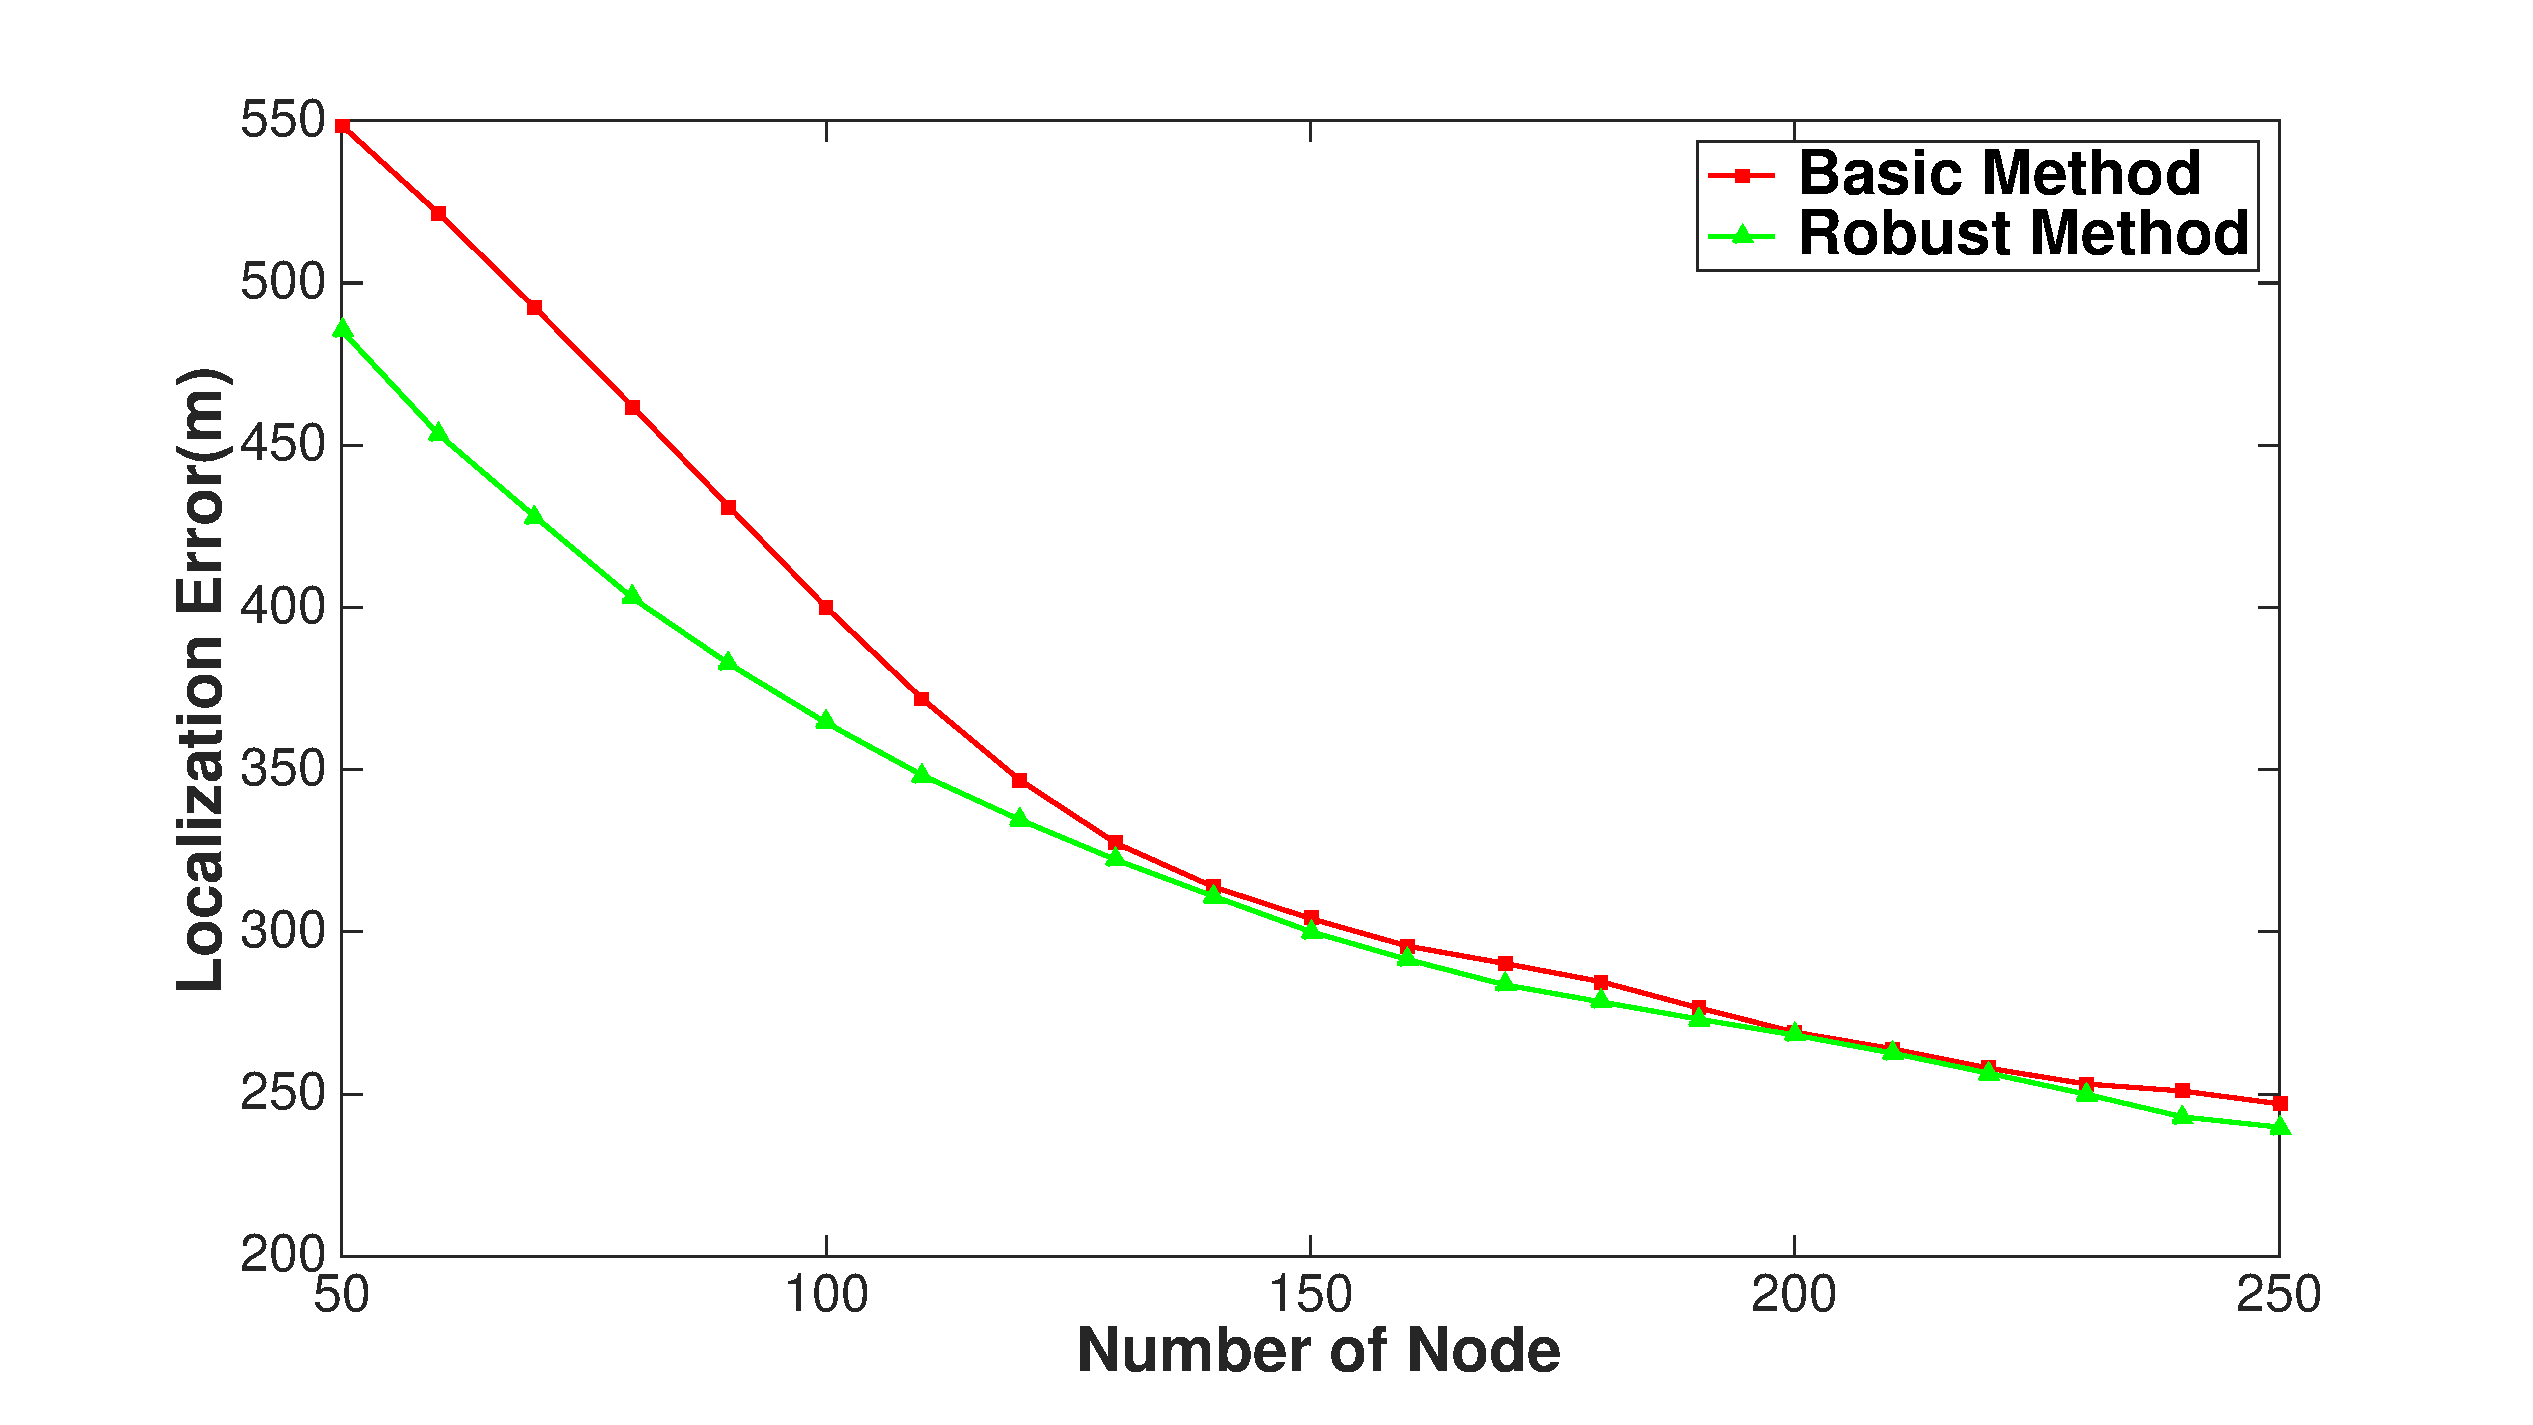
\includegraphics[scale=1.4,height=4.0cm]{image/Node_Number.eps}
     \vspace{2mm}
            \caption{Impact of number of nodes}
            \label{Node_Number}
            \vspace{-6mm}
  \end{figure}

\begin{figure}[hptb]
            \setlength{\abovecaptionskip}{0pt}
            \centering
            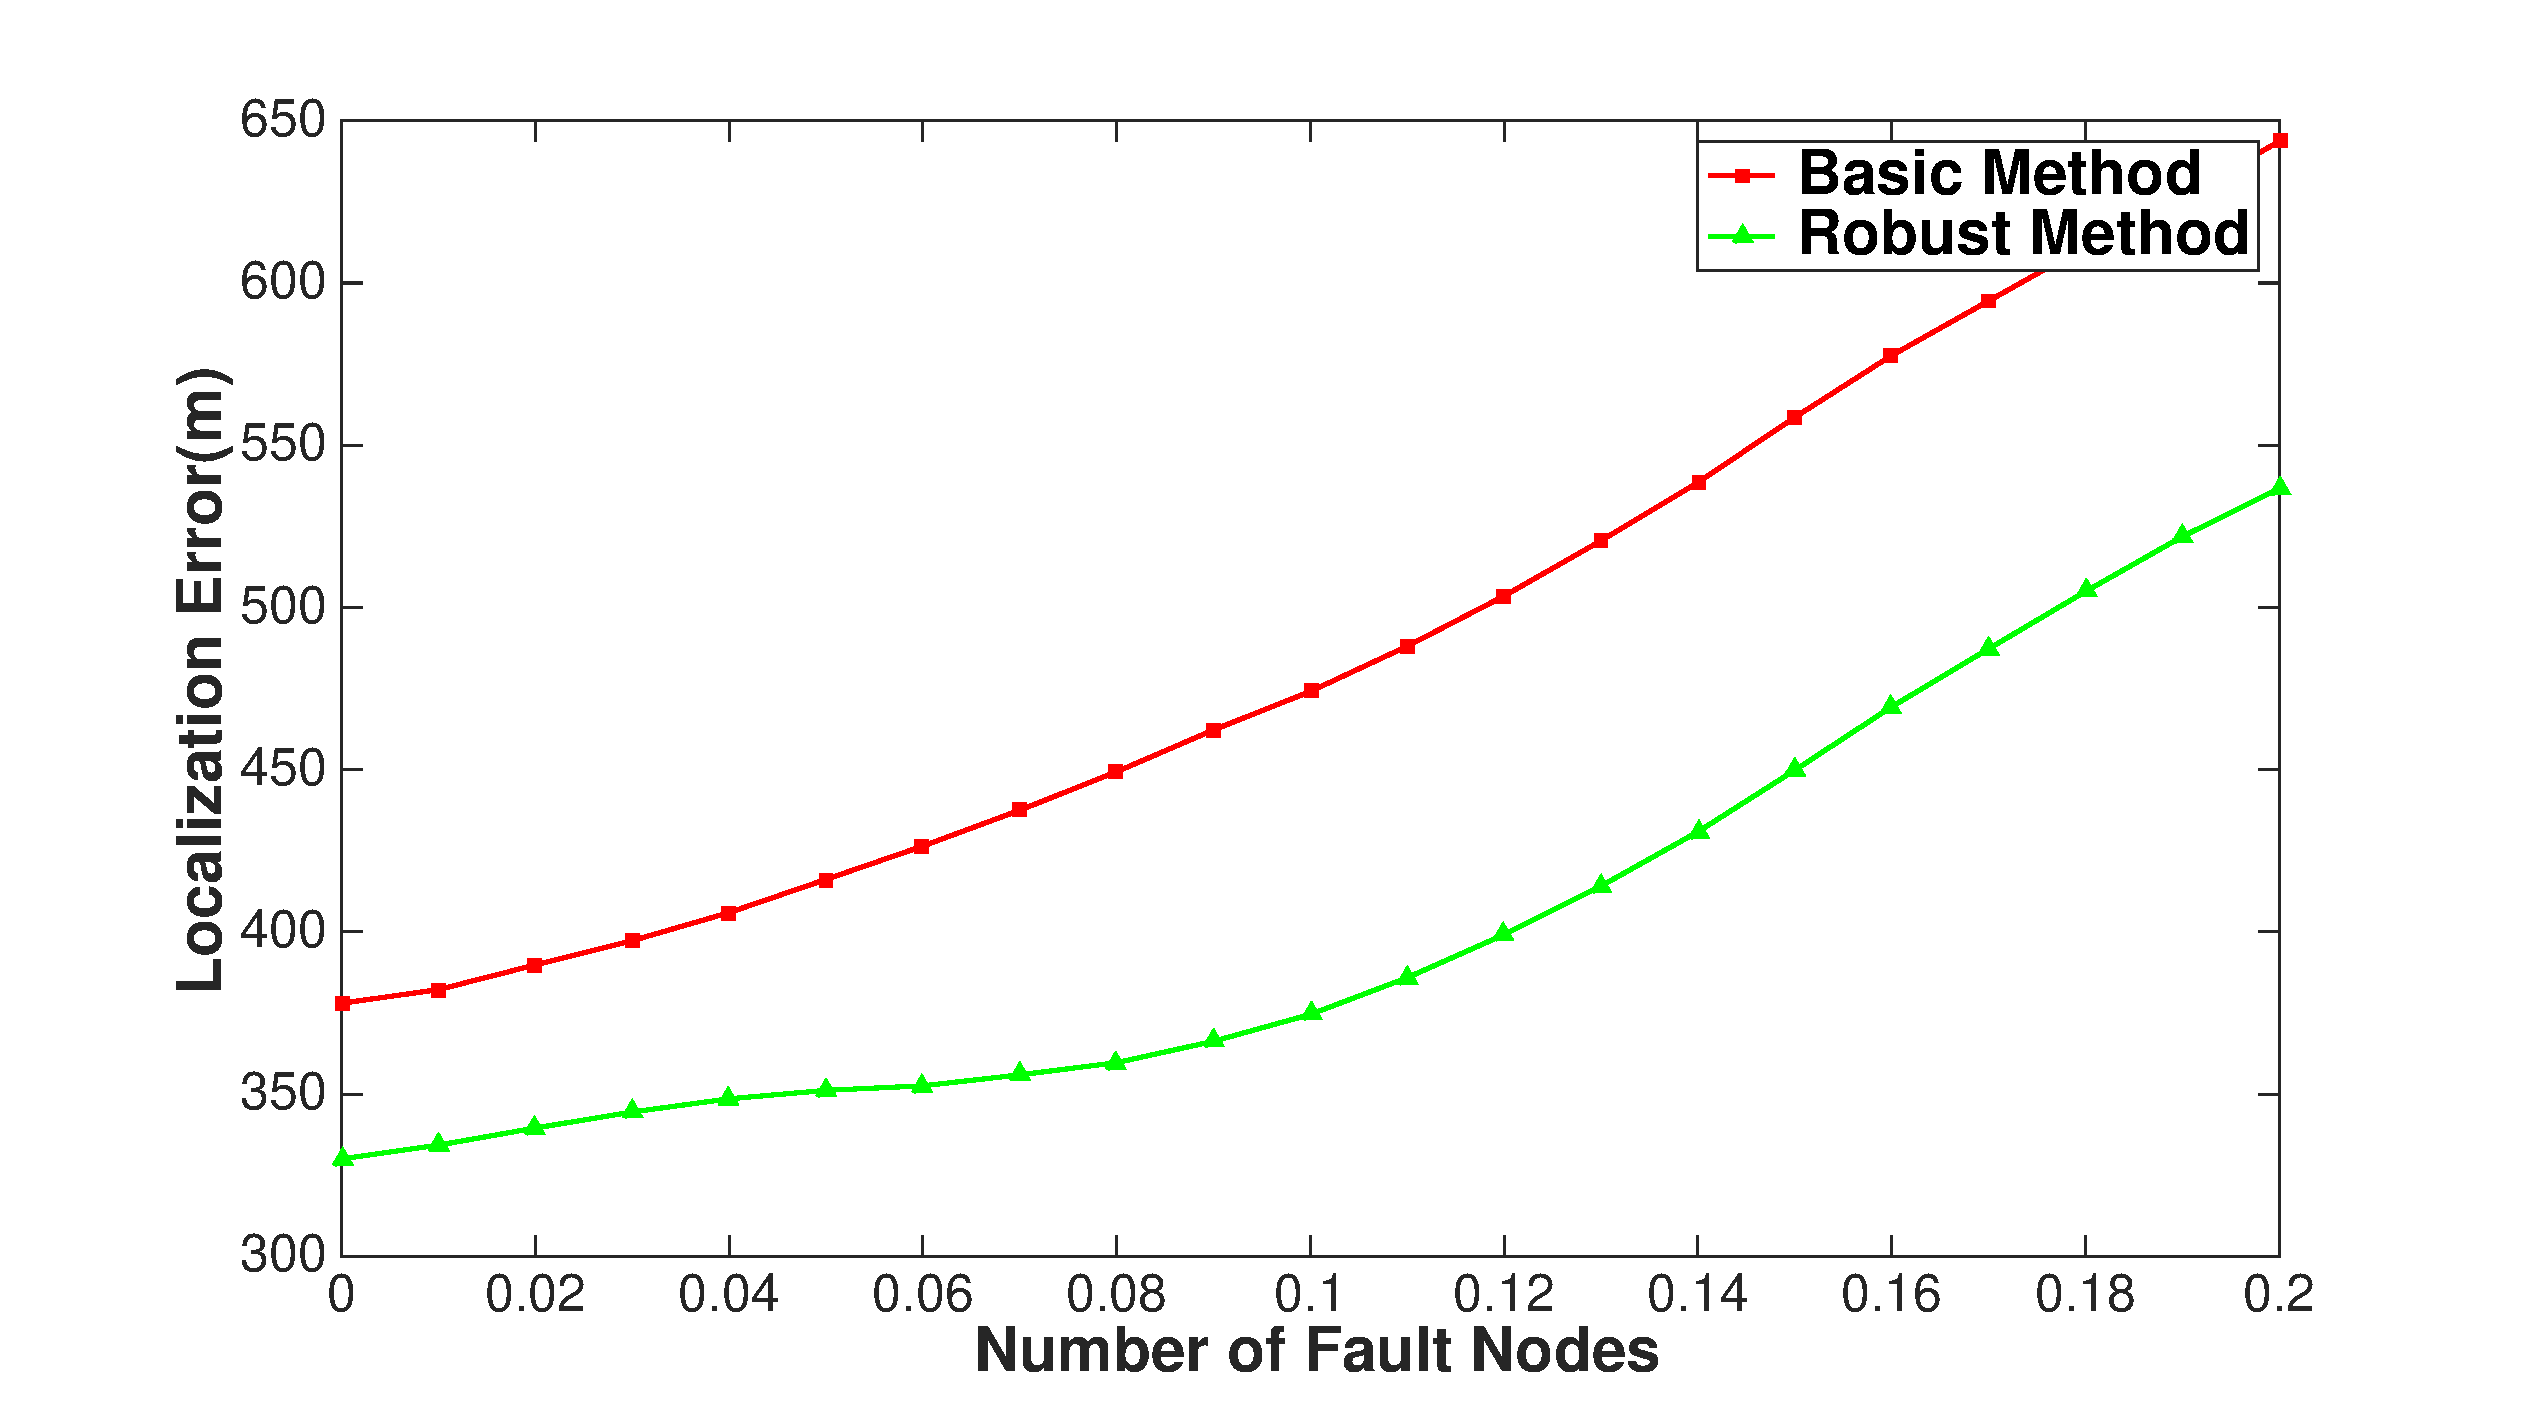
\includegraphics[scale=1.4,height=4.0cm]{image/Faulty_Node.eps}
     \vspace{2mm}
            \caption{Impact of number of error nodes.}
            \label{Faulty_Node}
            \vspace{-6mm}
  \end{figure}

  \begin{figure}[hpt]
            \setlength{\abovecaptionskip}{0pt}
            \centering
            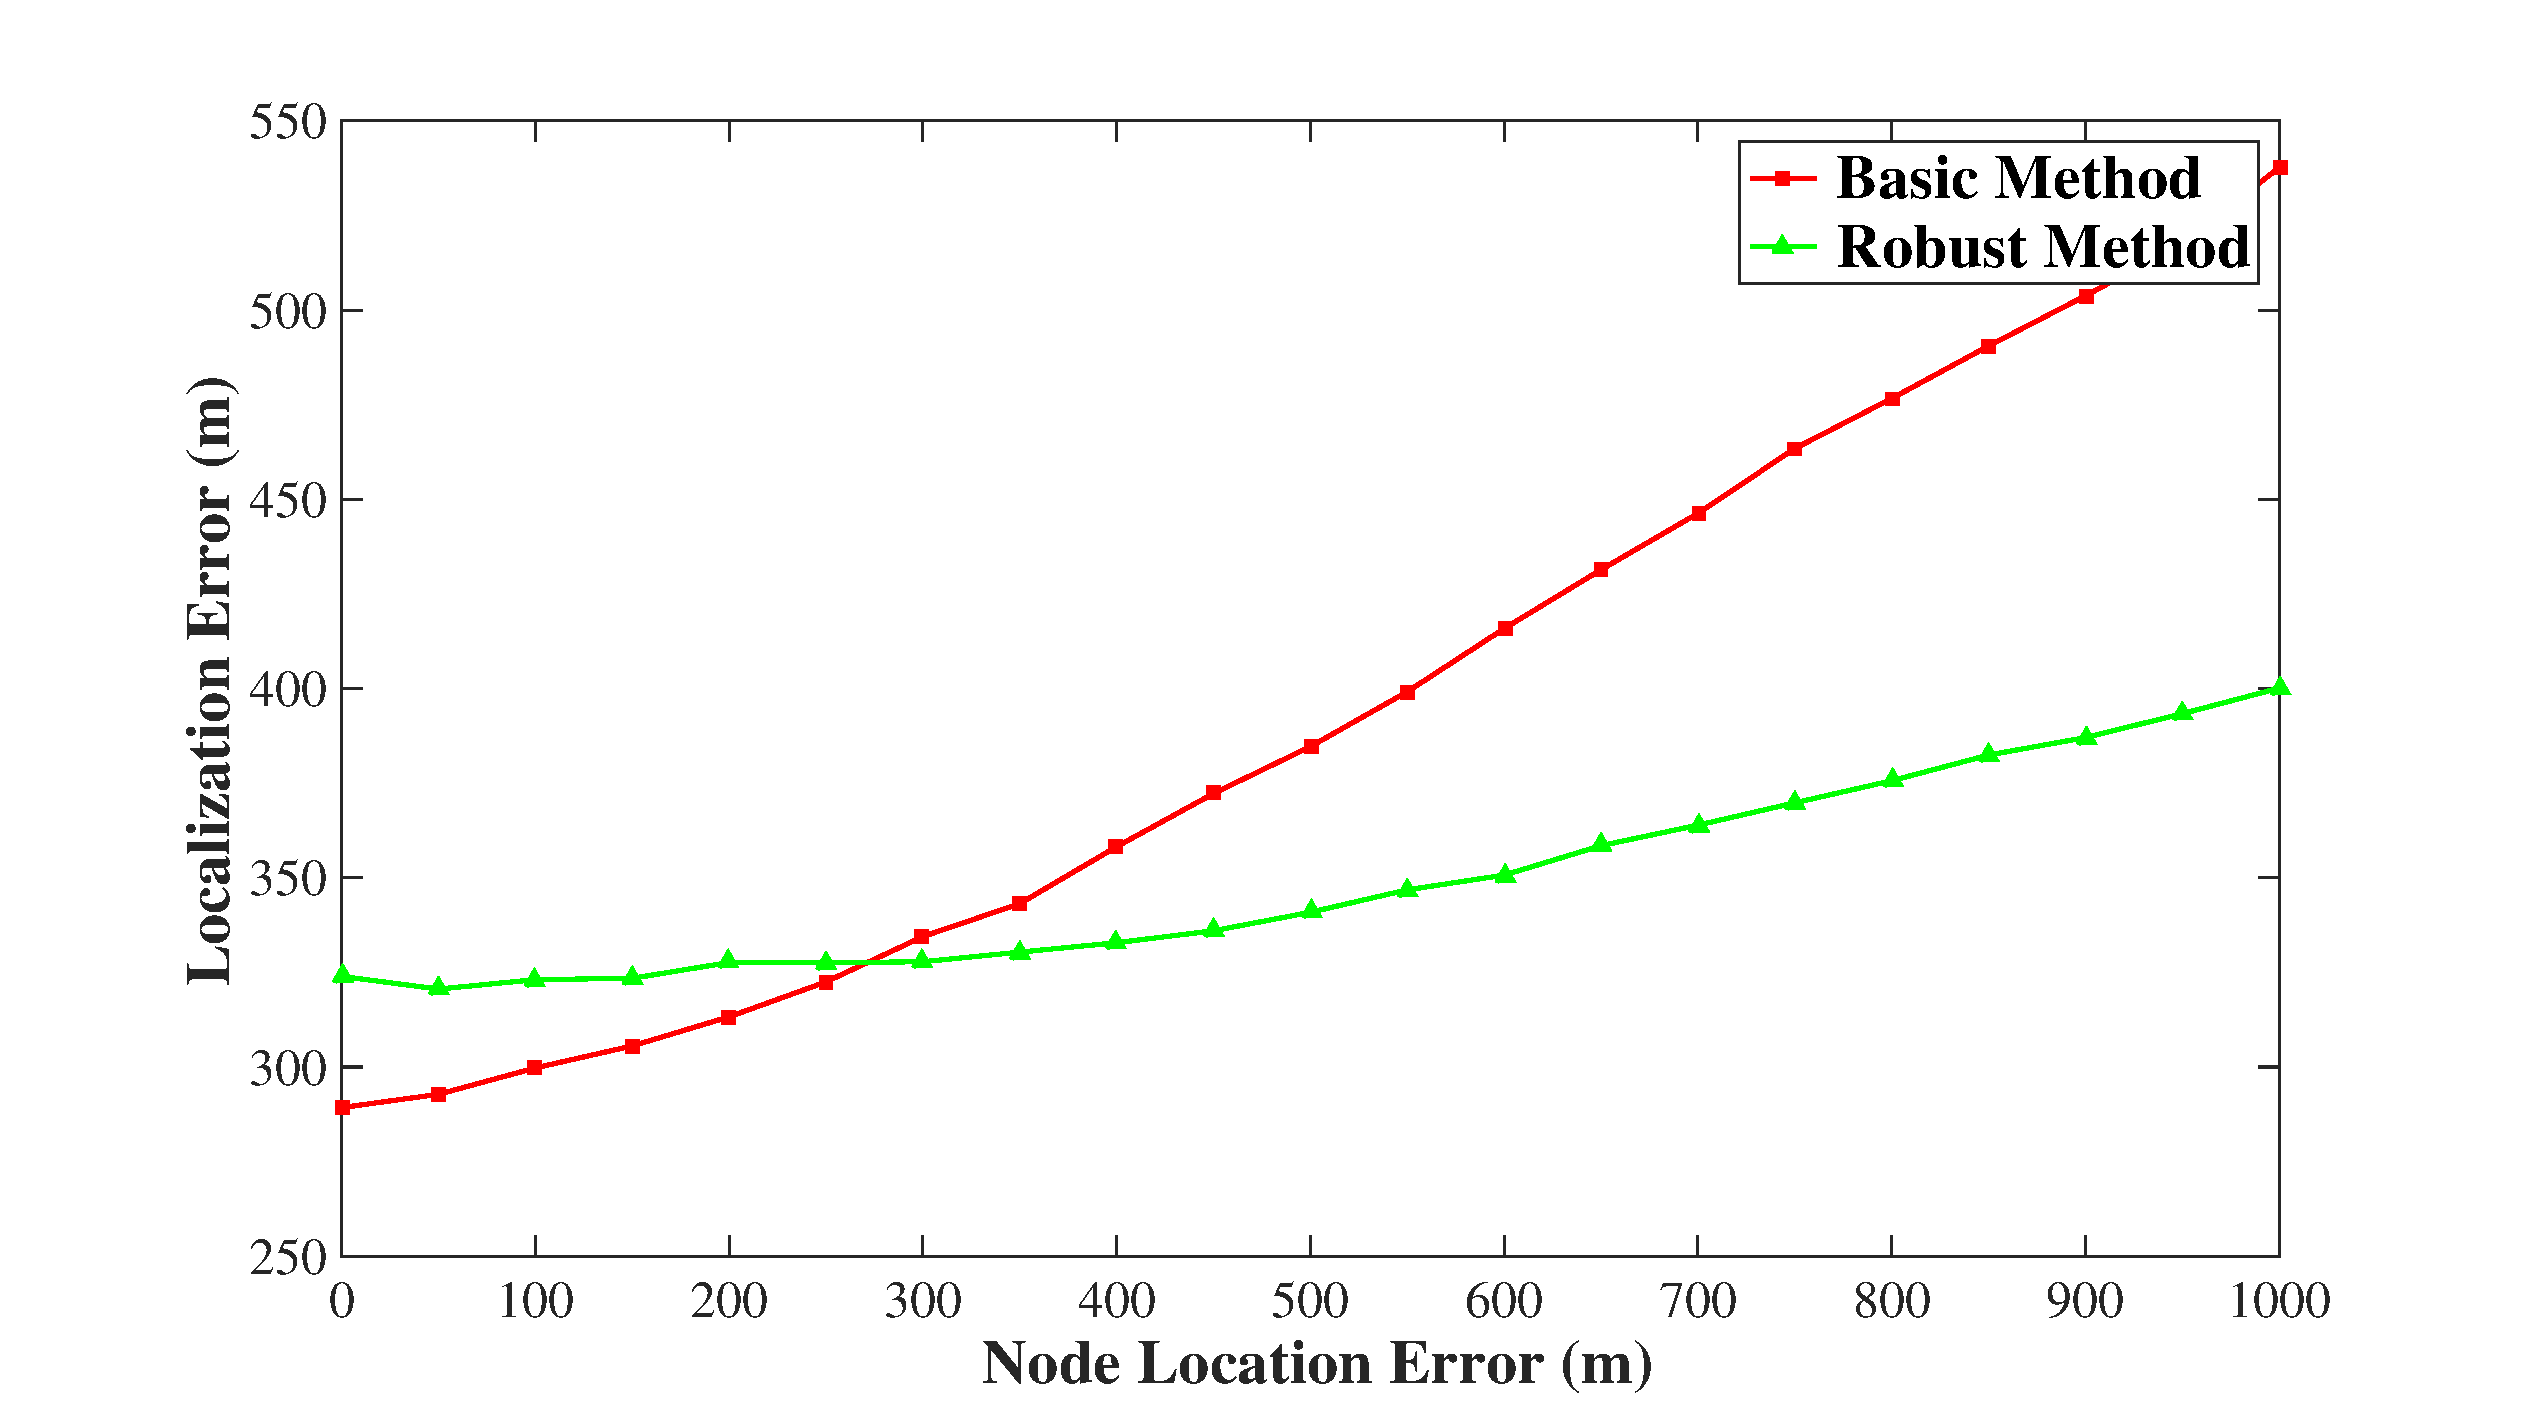
\includegraphics[scale=1.4,height=4.0cm]{image/Location.eps}
     \vspace{2mm}
            \caption{Impact of the position error.}
            \label{Location}
            \vspace{-6mm}
  \end{figure}
  
  \textbf{4) Impact of the orientations error of nodes:}
In the experiment, we evaluated the impact of the angle error of nodes for the basic ThunderLoc and robust ThunderLoc with the range from 0 to 20 degree in steps of 2. 
Other simulation parameters keep default.
As the orientations of nodes exist errors, we can guess the error of orientations may influence the localization accuracy. 
 As shown in Fig. \ref{Direction}, the graph to the localization error for the two methods is rising as the angle error of nodes increases. 
When the angle error of nodes is relative large, the average localization error for the robust ThunderLoc is much smaller than basic ThunderLoc, 
 so the localization accuracy of robust ThunderLoc is much better than that of basic ThunderLoc.
  \begin{figure}[hptb]
            \setlength{\abovecaptionskip}{0pt}
            \centering
            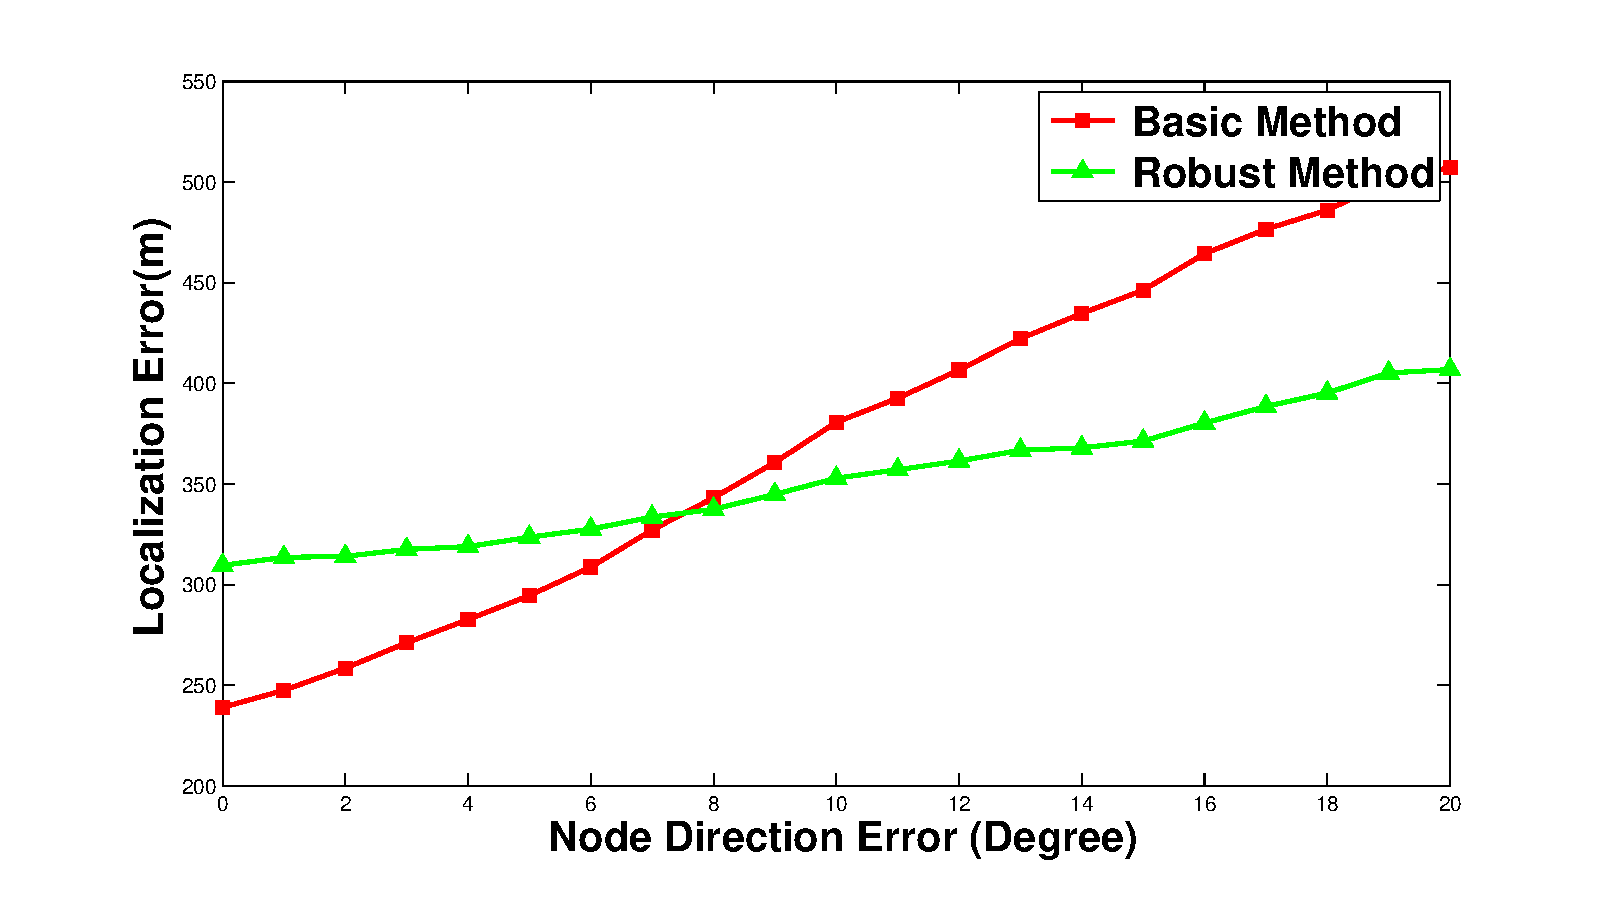
\includegraphics[scale=1.4,height=4.0cm]{image/Direction.eps}
     \vspace{2mm}
            \caption{Impact of orientation error.}
            \label{Direction}
            \vspace{-6mm}
  \end{figure}

 

 % \textbf{Summary:} From these experiments, we can get the following conclusions:

 % (1) The increase of the number of nodes can improve the localization accuracy, especially when we have many participants holding the mobile phones with different postures.

 % (2) The increase of the number of fault nodes can reduce the localization accuracy, and robust ThunderLoc is better than basic ThunderLoc when the percentage of fault nodes is above 0.06.

 % (3) The errors of node position and orientation can impact the localization error, the localization performance of robust ThunderLoc is better than basic ThunderLoc.

  \vspace{-4mm}
\subsection{3D Simulation}

The height of the thunder should be considered in some applications, such as lightning channel reconstruction. 
In this section, we evaluated our localization methods in the 3D scenario.  
In the simulation, we randomly deployed 100 dual-microphone smartphones to cover a 10km $\times$ 10km region. 
The altitude of mobile phones is about 10m and the height of the thunder is about 3km. 
The number of nodes is 100, and the angle error range of smartphones is 5.
Due to limitations on space, we just investigate the impact of the number of smartphones with the range from 80 to 160. 
The localization result of the experiment is showed in Fig. \ref{3D}.
Comparison with the 2D scenario, the localization errors are much larger in 3D space for the same number of smartphones. 
The reason is that the localization errors are related to the size of space grids divided by the perpendicular bisector of dual-microphone.
In the 3D scenario, the more smartphones is needed to achieve high-accuracy localization. 
%When the number of nodes is 120, the average localization error of robust ThunderLoc is about 800m.
  \begin{figure}[ht]%HT
            \setlength{\abovecaptionskip}{0pt}
            \centering
            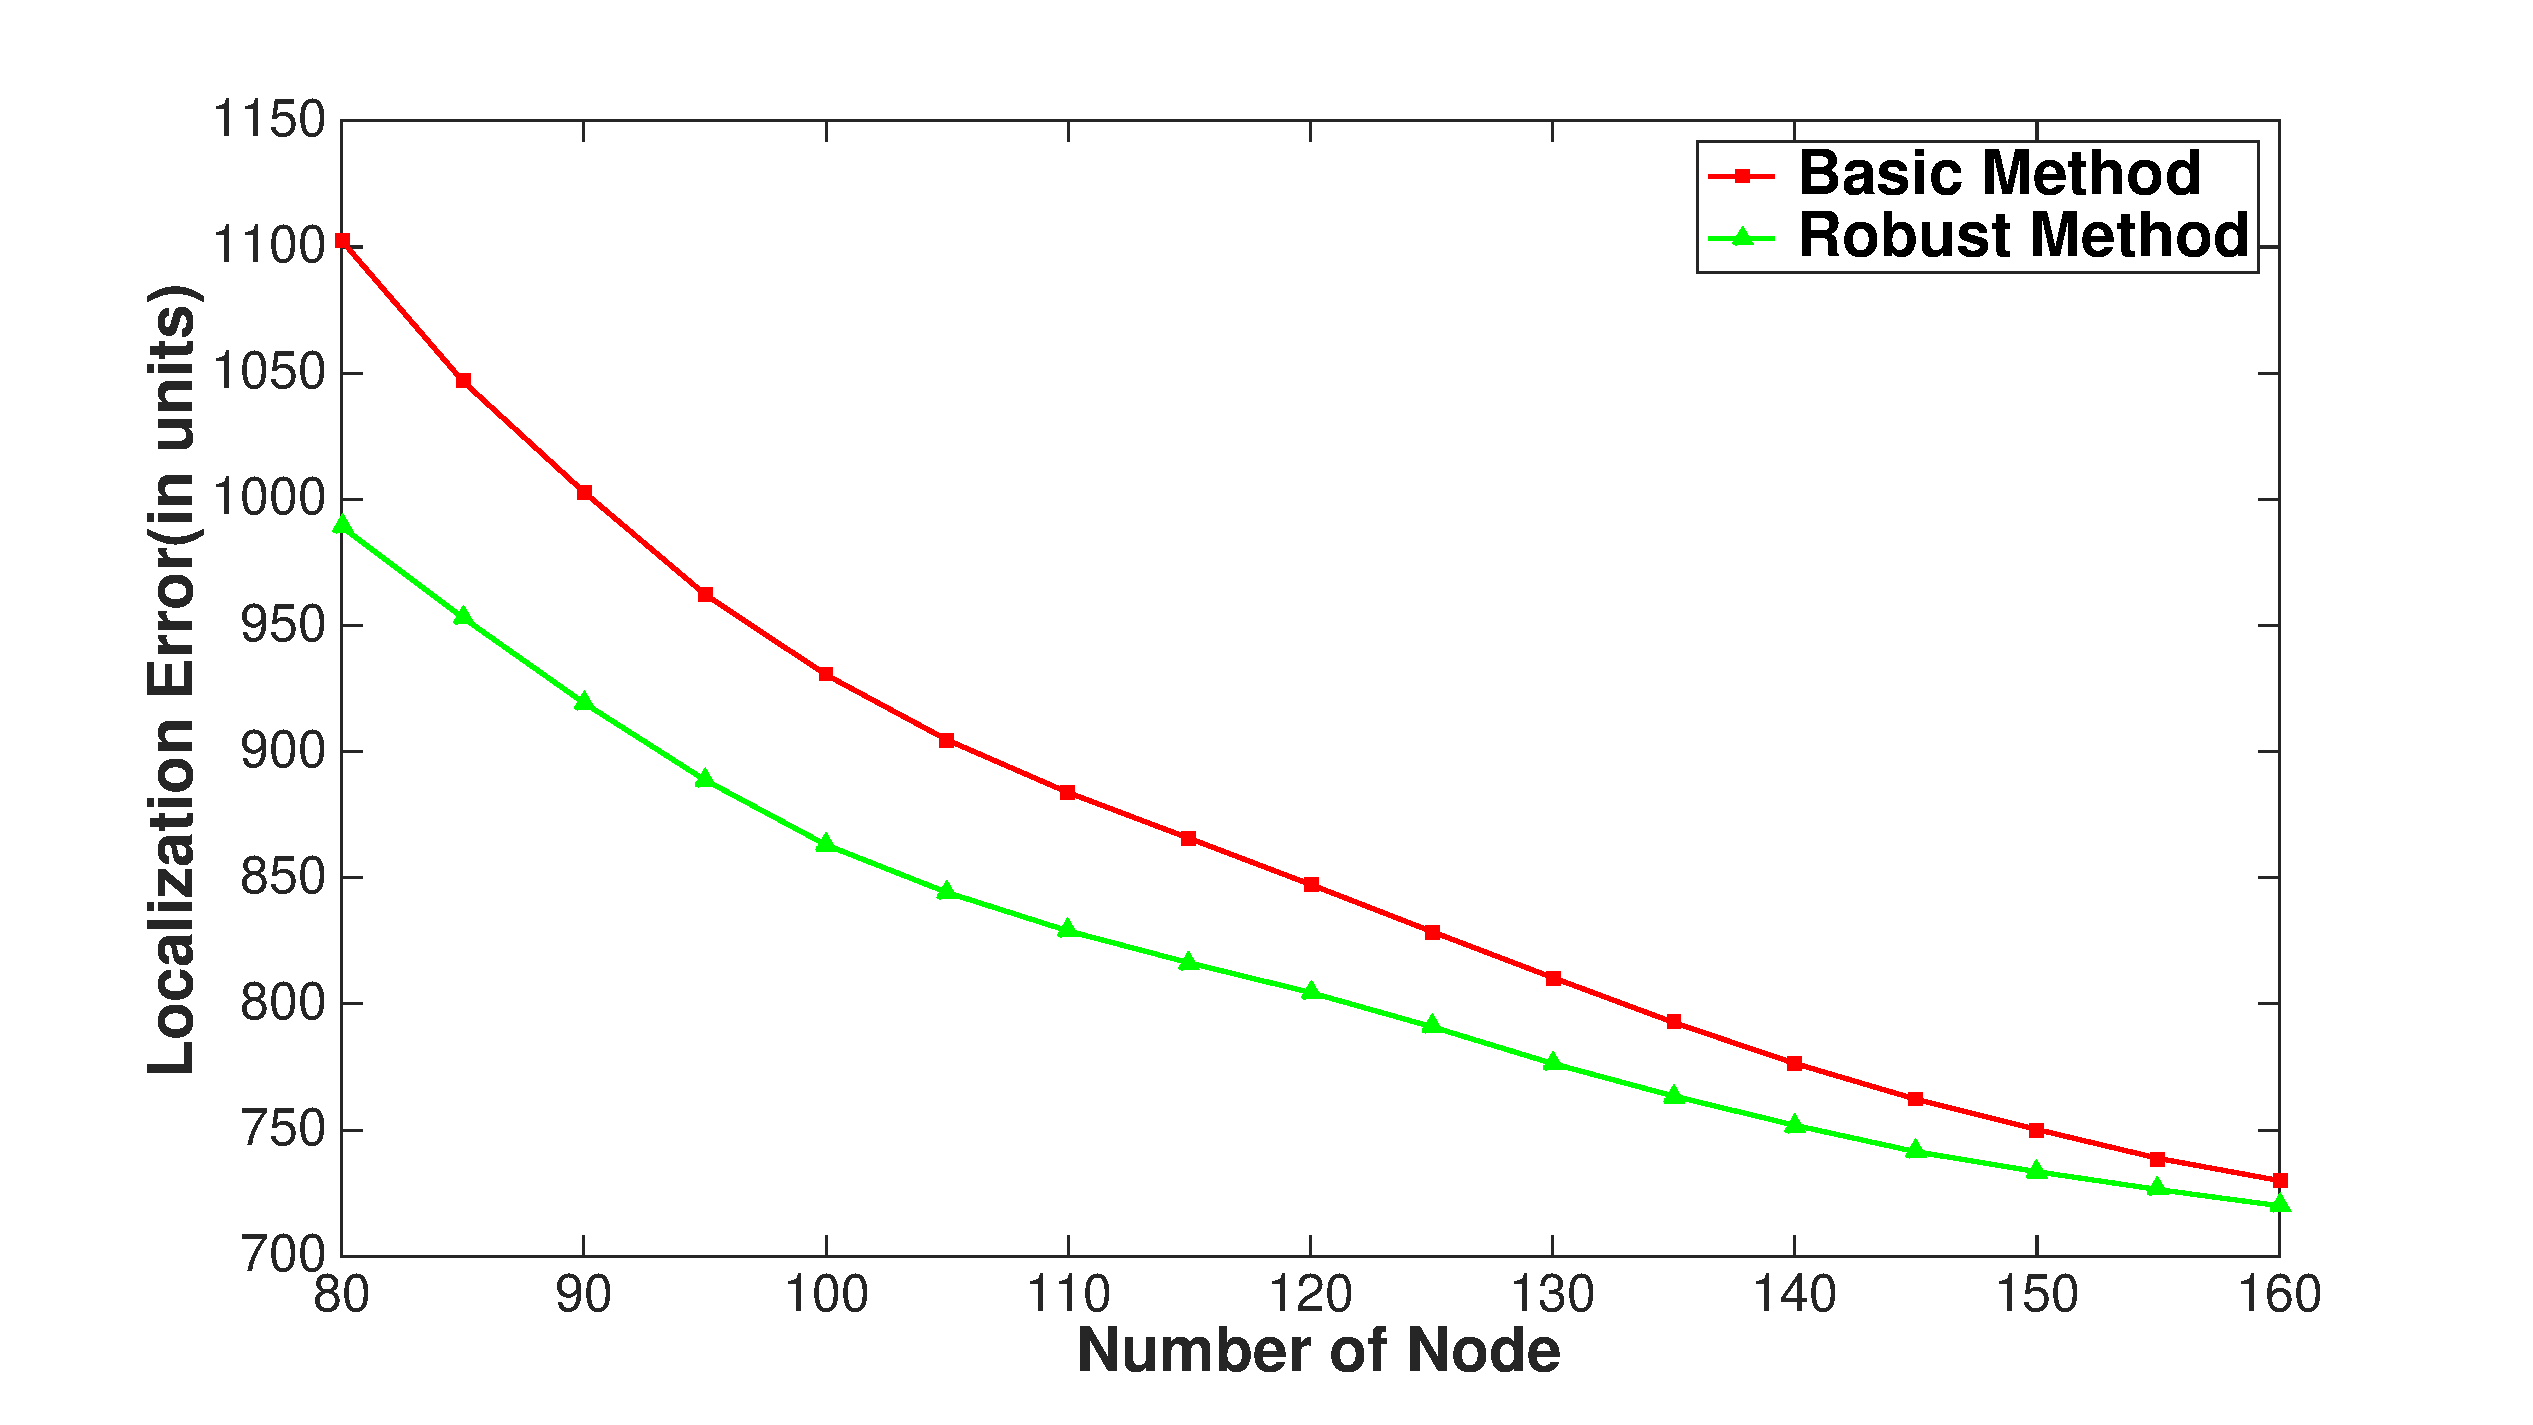
\includegraphics[scale=1.4,height=4.0cm]{image/3D.eps}
     \vspace{2mm}
    	   \caption{Thunder localization in 3D space}
            \label{3D}
            \vspace{-6mm}
  \end{figure}
  
\subsection{Virtual Thunder Emulation}

The virtual thunder test was useful as a proper verification of the functionality of our ThunderLoc project. 
We use 30 dual-microphone Xiaomi smartphones as sensor nodes and connect them through CISCO CVR328W-K9-CN wireless router. 
The distance between the two microphones is 14cm. We set the 30 nodes in a size of 1km$\times$1km space and there just one target during an experiment.
In order to simulate the thunder, we broadcast the recorded sound signal of thunder by speaker at the top of the three buildings. 
Smartphones are randomly deployed around the building.The localization results are shown in Fig. \ref{Virtual}, where blue squares stand for dual-microphone smartphones, and blue circles and red circles are the ground truth and the estimated position by robust localization method. 
An arrow originates from the estimated position to the real position of the virtual thunder. 
As the results shown in Fig. \ref{Virtual}, the estimated position is close to real position and the localization error is within the expected range,
which means that our proposed ThunderLoc system can effectively locate the thunder  by the way of crowdsensing.
  \begin{figure}[ht]
            \setlength{\abovecaptionskip}{0pt}
            \centering
            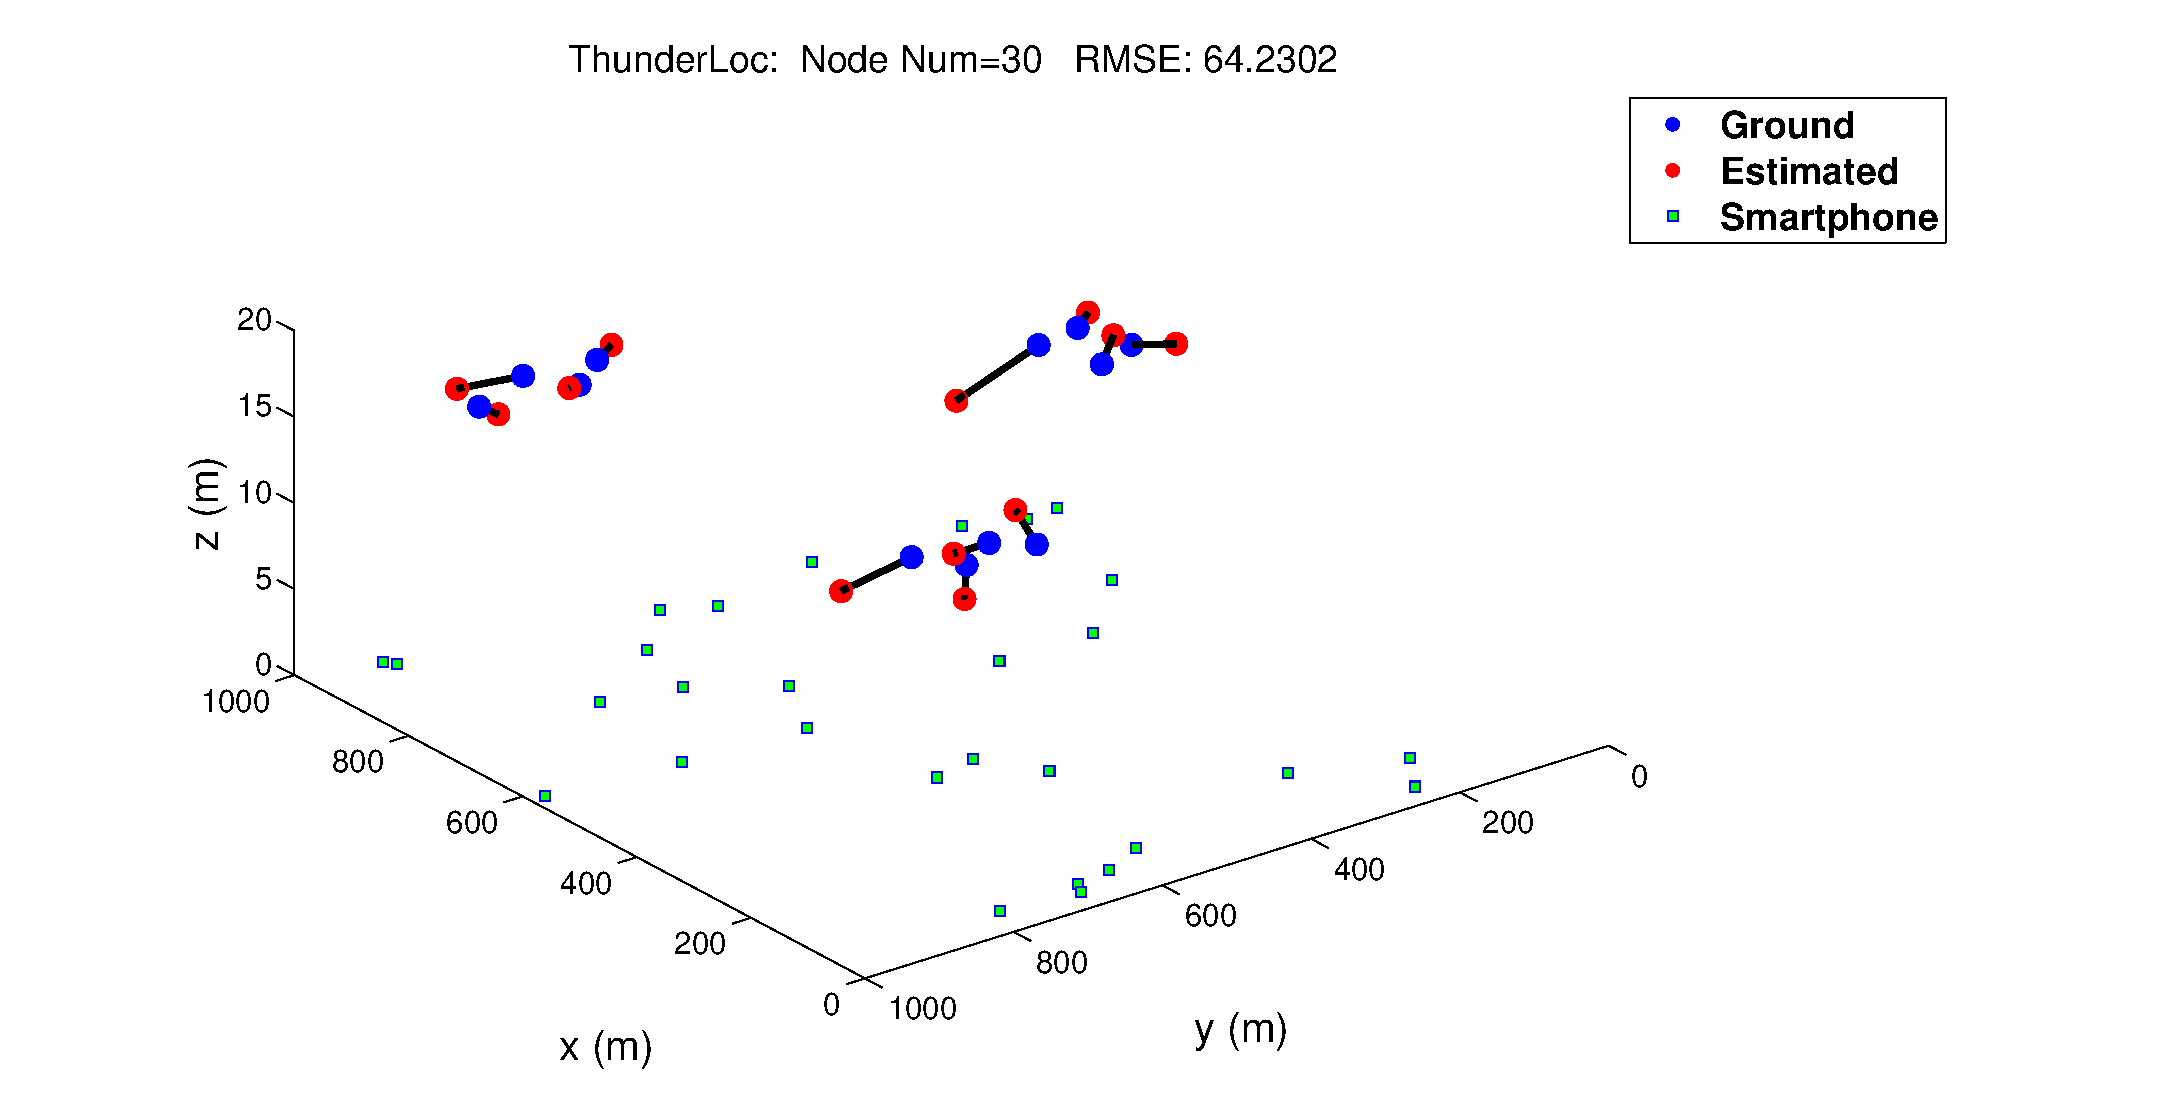
\includegraphics[scale=2,height=4.5cm]{image/virtual.eps}
     \vspace{2mm}
            \caption{Experiment result.}
            \label{Virtual}
            \vspace{-8mm}
  \end{figure}


